%\documentclass{beamer} %voce pode usar este modelo tambem
\documentclass[t,handout,9pt]{beamer}
\usepackage{graphicx}
\usepackage{url}
\usepackage[british]{babel}
%\batchmode
% \pgfpagesuselayout{4 on 1}[letterpaper,landscape,border shrink=5mm]
\usepackage{amsmath}
\usepackage{amssymb}
\usepackage{amsfonts}
\usepackage{enumerate}
\usepackage{epsfig}
\usepackage{bbm}
\usepackage{calc}
\usepackage{adjustbox}
\usepackage{color}
\usepackage{ifthen}
\usepackage{capt-of}
\usepackage{float}
\usepackage{booktabs}
\usepackage{dcolumn}
\usepackage{multicol}
\usepackage{hyperref}
\usepackage[flushleft]{threeparttable}
\usepackage{subcaption}
\usepackage{adjustbox}
\usepackage{ragged2e}
\usepackage{pgfpages}
\usepackage{multirow}
%\usepackage{showframe}

\usepackage{cmbright}

\renewcommand\ttdefault{cmvtt} % selects CM typewriter

\usepackage[utf8]{inputenc} % Required for inputting international characters
\usepackage[T1]{fontenc} 	% Output font encoding for international characters

%\DeclareFontShape{OT1}{cmss}{b}{n}{<->ssub * cmss/bx/n}{}

\usetheme[compress]{Berlin}
\definecolor{sapienza}{RGB}{0, 49, 83}
\usecolortheme[named=sapienza]{structure}

\usepackage[backend=bibtex,style=alphabetic,giveninits=true,url=false,eprint=false,doi=false]{biblatex}
\DeclareNameAlias{sortname}{last-first}
\renewcommand*{\nameyeardelim}{\addcomma\addspace}
\renewcommand*{\bibfont}{\footnotesize}
\addbibresource{example.bib}
\setbeamerfont{footnote}{size=\tiny}

\setbeamerfont{title}{size=\LARGE}

% reduce spaces between tables/figures and caption
\usepackage[font=small,skip=1pt]{caption}

%% pgf plots stuff
%\usepackage{pgfplots}
%\pgfplotsset{compat=newest}
%% the following commands are needed for some matlab2tikz features
%\usetikzlibrary{plotmarks}
%\usetikzlibrary{arrows.meta}
%\usepgfplotslibrary{patchplots}

% one navigation dot per slide trick
\AtBeginSection[]{\subsection{}}

% fix misbehave for allowframebreaks
\usepackage{etoolbox}
\makeatletter
\patchcmd{\slideentry}{\ifnum#2>0}{\ifnum2>0}{}% replace the subsection number test with a test that always returns true
% use frame numbers instead of subsection slide numbers so that frames broken over slides get separate circles
\patchcmd{\slideentry}{\c@subsectionslide}{\c@framenumber}{}{\@error{unable to patch}}
\patchcmd{\beamer@writeslidentry}{\c@subsectionslide}{\c@framenumber}{}{\@error{unable to patch}}

% date in footer trick
\makeatletter
  \setbeamertemplate{footline}{%
    \begin{beamercolorbox}[colsep=1.5pt]{upper separation line foot}
    \end{beamercolorbox}
    \begin{beamercolorbox}[ht=2.5ex,dp=1.125ex,%
      leftskip=.3cm,rightskip=.3cm plus1fil]{author in head/foot}%
      \leavevmode{\usebeamerfont{author in head/foot}\insertshortauthor}%
      \hfill%
      {\usebeamerfont{institute in head/foot}\usebeamercolor[fg]{institute in head/foot}\insertshortinstitute}%
    \end{beamercolorbox}%
    \begin{beamercolorbox}[ht=2.5ex,dp=1.125ex,%
      leftskip=.3cm,rightskip=.3cm plus1fil]{title in head/foot}%
      {\usebeamerfont{title in head/foot}\insertshorttitle\hfill\insertshortdate}%
    \end{beamercolorbox}%
    \begin{beamercolorbox}[colsep=1.5pt]{lower separation line foot}
    \end{beamercolorbox}
  }
\makeatletter

% remove dot for titlepage and Outline
\makeatletter
\let\old@beamer@writeslidentry\beamer@writeslidentry
\def\beamer@writeslidentry{%
  \expandafter\beamer@ifempty\expandafter{\beamer@framestartpage}{}% does not happen normally
  {%else
    \clearpage\beamer@notesactions%
  }
}
\makeatother

% let's number figure captions
\setbeamertemplate{caption}[numbered]

% trick for grouping equations
\newenvironment{rcases}
  {\left.\begin{aligned}}
  {\end{aligned}\right\rbrace}

%-------------------------Titulo/Autores/Orientador------------------------------------------------
\title[Introduction to Computer Programming]{Introduction to Computer Programming}
\date[A.Y. 2024-2025]{\\A.Y. 2024-2025}
\author[Alessio Martino]{Prof. Alessio Martino\\
\smallskip
{\small \href{mailto:amartino@luiss.it}{\texttt{amartino@luiss.it}}}\\
\smallskip
}
\institute[11/09/2024]{Department of Business and Management\\Viale Romania 32, 00197 Rome\\[\bigskipamount]

\includegraphics[scale=0.4]{Figures/cliente-luiss.png}%
}

%-------------------------Logo na parte de baixo do slide------------------------------------------
%\pgfdeclareimage[height=0.7cm]{senac-logo}{senac-logo.pdf}
%\logo{\pgfuseimage{senac-logo}\hspace*{0.5cm}}

%-------------------------Este código faz o menuzinho bacana na parte superior do slide------------
%\AtBeginSection[]
%{
%  \begin{frame}<beamer>
%    \frametitle{Outline}
%    \tableofcontents[currentsection]
%  \end{frame}
%}
%\beamerdefaultoverlayspecification{<+->}
% -----------------------------------------------------------------------------

\begin{document}
% -----------------------------------------------------------------------------

%---Gerador de Sumário---------------------------------------------------------

\frame[noframenumbering]{
	\titlepage
}

% begin personalization stuff
\setbeamertemplate{navigation symbols}{%
	\insertslidenavigationsymbol
	\insertframenavigationsymbol
	\insertsubsectionnavigationsymbol
	\insertsectionnavigationsymbol
	\insertdocnavigationsymbol
	\insertbackfindforwardnavigationsymbol
	\hspace{1em}%
	\usebeamerfont{footline}
	\insertframenumber/\inserttotalframenumber%
}
\setbeamertemplate{itemize items}[circle]
\setbeamertemplate{enumerate items}[circle]
\setbeamertemplate{bibliography item}{\insertbiblabel}
% end personalization stuff

\section[]{}
\begin{frame}{Outline}
	\tableofcontents
\end{frame}
%\begin{frame}{Outline}
%\begin{multicols}{2}
%  \tableofcontents
%\end{multicols}
%\end{frame}
%---Fim do Sumário------------------------------------------------------------

% reset navigation dots for other slides
\makeatletter
\let\beamer@writeslidentry\old@beamer@writeslidentry
\makeatother

% -----------------------------------------------------------------------------
\section{Introduction to Python}
\begin{frame}{Introduction to Python}
\begin{center}Why Python?\end{center}
\vfill
\begin{itemize}
	\item A \textcolor{red}{high-level} language for \textcolor{red}{beginners}
	\item with a \textcolor{red}{clean syntax}, but...
	\item \textcolor{red}{Industrial strength} programming language used at thousands of companies (one of three official Google languages)
	\item Free, well documented, well supported
\end{itemize}
\vfill
\begin{block}{Recall}
We will use Python 3 (there are non-backwards compatible differences with respect to Python 2). Further, Python 2 is now unsupported.
\end{block}
\vfill
\end{frame}
%
\begin{frame}
\vfill
A (Python) program is composed by a sequence of:
\begin{itemize}
	\item \textcolor{red}{definitions} (also \textcolor{red}{expressions}) which are \textcolor{red}{evaluated}
	\item \textcolor{red}{statements} (also \textcolor{red}{commands}) which are \textcolor{red}{executed}
\end{itemize}
\vfill
In plain terms...
\begin{itemize}
	\item \textcolor{red}{expressions} yield some results (e.g., \texttt{5 * 5})
	\item \textcolor{red}{statements} instruct the interpreter to do something (e.g., print on screen, assign to variable)
\end{itemize}
\vfill
Expressions and statements can either
\begin{itemize}
	\item be directly written into a shell (\textcolor{red}{interactive mode})
	\item be written into a text file and then loaded into the shell (\textcolor{red}{script mode}).
\end{itemize}
\vfill
\end{frame}
%
\begin{frame}
\begin{center}Interactive vs. Script Mode\end{center}
\begin{description}
	\item[Interactive Mode:] perfectly fine for testing and learning.\\
	Type your commands/expressions into the shell and Python will execute/evaluate those immediately:
	\begin{table}[]
	\begin{tabular}{ll}
	\texttt{>{}>{}> 5 * 5} & $\leftarrow$input  \\
	\texttt{25}        & $\leftarrow$output
	\end{tabular}
	\end{table}
 	\item[Script Mode:] is what you normally do.\\
 	\begin{itemize}
 		\item write the entire source code in a text file ending with the \texttt{.py} extension (say \texttt{myscript.py})
 		\item \texttt{myscript.py} will be executed in its entirety by the Python interpreter
 	\end{itemize}
\end{description}
\end{frame}
%
\section{Programming in Python}
\begin{frame}{Programming in Python}
\adjustbox{valign=t}{\begin{minipage}{0.4\textwidth}
\begin{itemize}
\item programs manipulate \textcolor{red}{data objects}
\item each data object has its own \textcolor{red}{type}, which defines the type of operations that can be done with them
\item objects can either be:
	\begin{description}
		\item[Scalar:] cannot be subdivided
		\item[Non-scalar:] have an inner structure that can be accessed
	\end{description}
\end{itemize}
\end{minipage}}%
\hfill
\adjustbox{valign=t}{\begin{minipage}[t]{0.6\textwidth}
\vspace{0.5cm}
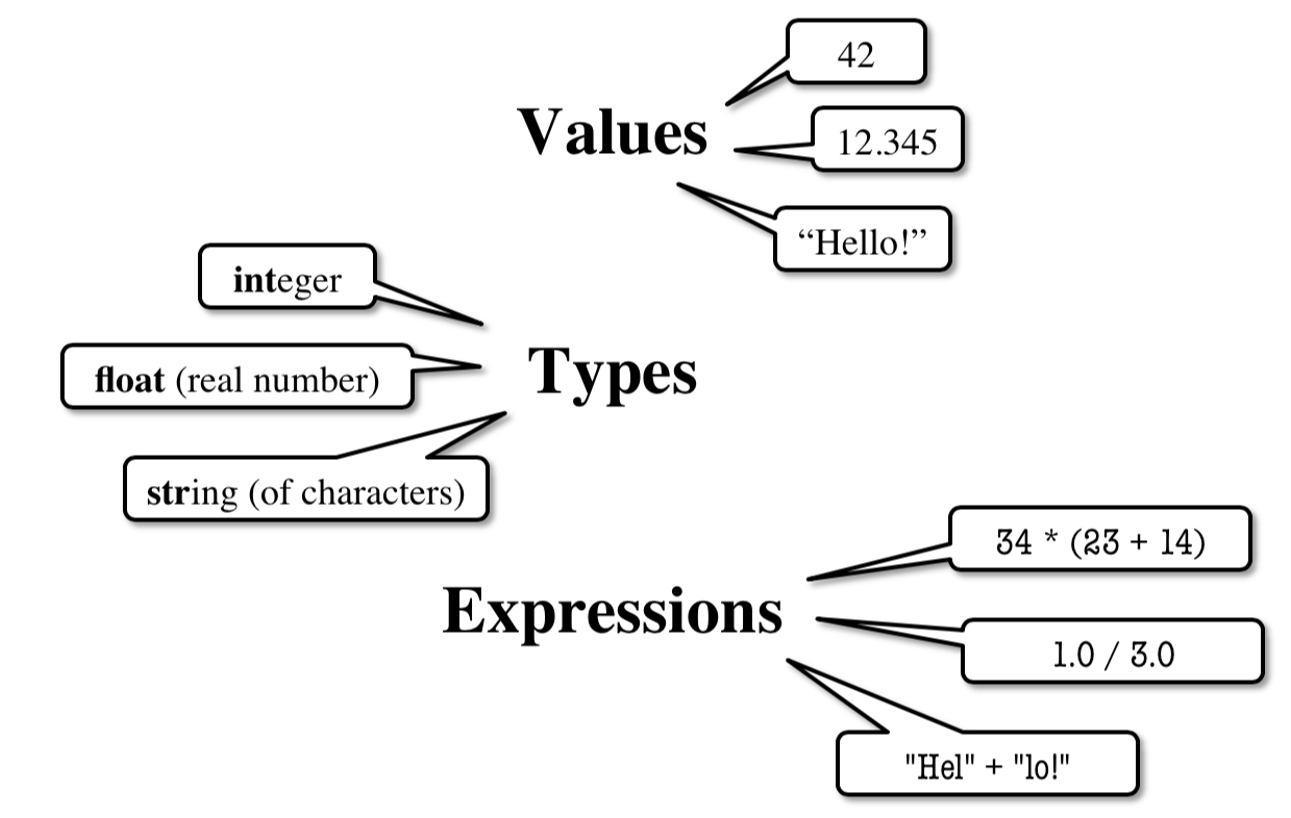
\includegraphics[width=\textwidth]{Figures/PythonBasics}
\end{minipage}}
\end{frame}
%
\section{Scalar Objects}
\begin{frame}{Scalar Objects}
\begin{itemize}
	\item \texttt{int}: represents integers (e.g., \texttt{5})
	\item \texttt{float}: represents real numbers (e.g., \texttt{3.14})
	\item \texttt{bool}: represents Boolean values (\texttt{True} or \texttt{False})
	\item \texttt{NoneType}: special with only one value (\texttt{None})
\end{itemize}
\begin{block}{Hint}
Use the \texttt{type()} function if you are not sure about the data type.
\end{block}
Examples:
\begin{table}[]
\begin{tabular}{ll}
\texttt{>{}>{}> type(109)} & $\leftarrow$input  \\
\texttt{<class 'int'>}        & $\leftarrow$output
\end{tabular}
\end{table}
\begin{table}[]
\begin{tabular}{ll}
\texttt{>{}>{}> type(10.9)} & $\leftarrow$input  \\
\texttt{<class 'float'>}        & $\leftarrow$output
\end{tabular}
\end{table}
\end{frame}
%
\subsection{Type \texttt{int()}}
\begin{frame}
Values:\\
\qquad $\ldots, -3, -2, -1, 0, 1, 2, 3, \ldots$\\
Integer literals look like a sequence of numbers with no periods nor commas.\\
Operations:\\
\begin{itemize}
	\item +, -, *, \slash \hfill [plain arithmetic]
	\item ** \hfill [to the power of]
	\item unary - \hfill [negative numbers]
	\item \% \hfill [modulo, remainder]
\end{itemize}
\begin{block}{Note}
In Python 3, operations between integers may not yield an integer.
\end{block}
Examples:
\begin{table}[]
\begin{flushleft}
\begin{tabular}{ll}
\texttt{>{}>{}> 7/5} & $\leftarrow$input  \\
\texttt{1.4}        & $\leftarrow$output\\
\texttt{>{}>{}> 7//5} & $\leftarrow$ \texttt{//} is the floor division!  \\
\texttt{1}        & %$\leftarrow$output
\end{tabular}
\end{flushleft}
\end{table}
\end{frame}
%
\subsection{Type \texttt{float()}}
\begin{frame}
Values:\\
\qquad some (approximated) range of $\mathbb{R}$\\
Note that:\\
\begin{itemize}
	\item numbers with a "\texttt{.}" are decimals (e.g., \texttt{2.0})
	\item numbers with no decimal separator are integers (e.g., \texttt{2})
\end{itemize}
Operations:\\
\begin{itemize}
	\item +, -, *, \slash \hfill [plain arithmetic]
	\item ** \hfill [to the power of]
	\item unary - \hfill [negative numbers]
	\item \% \hfill [modulo, remainder]
\end{itemize}
\begin{block}{Note}
In Python 3, operations between floats or between a float and an integer, always yield a float.
\end{block}
Indeed:
\begin{table}[]
\begin{flushleft}
\begin{tabular}{ll}
\texttt{>{}>{}> 7.0/5.0} & $\leftarrow$input  \\
\texttt{1.4}        & $\leftarrow$output\\
\texttt{>{}>{}> 7.0//5} & $\leftarrow$ \texttt{//} is the floor division!  \\
\texttt{1.0}        & %$\leftarrow$output
\end{tabular}
\end{flushleft}
\end{table}
\end{frame}
%
\begin{frame}
Python stores floating point numbers as base 2 (binary) fractions:
\begin{equation*}
	\text{\{number\}} = \text{\{integer mantissa\}} \cdot 2^{-\text{\{exponent\}}}
\end{equation*}
For example: $0.125 = 1 \cdot 2^{-3} = 1\cdot \frac{1}{2^3}=1\cdot \frac{1}{8}$.
\begin{block}{Warning}
Not all numbers can be represented in base 2 fractions. Python chooses the best approximation it can. The same also holds for some numbers in base 10 fraction. What about 1/3?
\end{block}
Python may yield some \textcolor{red}{approximation errors}, that propagate as expressions go through.\\
Example:
\begin{table}[]
\begin{flushleft}
\begin{tabular}{ll}
\texttt{>{}>{}> 0.1+0.2} & $\leftarrow$input  \\
\texttt{0.30000000000000004}        & $\leftarrow$output\\
\texttt{>{}>{}> 0.1+0.2+0.1+0.2} & \\
\texttt{0.6000000000000001}        & \\
\texttt{>{}>{}> 0.1+0.2+0.1+0.2+0.1+0.2+0.1+0.2} & \\
\texttt{1.2000000000000002}        & %$\leftarrow$output
\end{tabular}
\end{flushleft}
\end{table}
\end{frame}
%
\subsection{Type \texttt{bool}}
\begin{frame}
Values:\\
\qquad \texttt{True} and \texttt{False} (capitalized!)\\
Operations:\\
\begin{itemize}
	\item not \texttt{a} = $\begin{cases}
		\texttt{True} & \text{if} \texttt{ a } \text{is} \texttt{ False }\\
		\texttt{False} & \text{if} \texttt{ a } \text{is} \texttt{ True }
	\end{cases}$ \hfill [NOT operator]
	\item \texttt{a} and \texttt{b} = $\begin{cases}
		\texttt{True} & \text{if both} \texttt{ b } \text{and} \texttt{ a } \text{are} \texttt{ True}\\
		\texttt{False} & \text{otherwise}
	\end{cases}$ \hfill [AND operator]
	\item \texttt{a} or \texttt{b} = $\begin{cases}
		\texttt{True} & \text{if} \texttt{ a } \text{is} \texttt{ True } \text{or} \texttt{ b } \text{is} \texttt{ True }\\
		\texttt{False} & \text{otherwise}
	\end{cases}$ \hfill [OR operator]
\end{itemize}
Booleans are the output of comparisons between items (e.g., \texttt{int} or \texttt{float}):
\begin{description}
	\item[Order:] \texttt{i<j}, \texttt{i>j}, \texttt{i<=j}, \texttt{i>=j}
	\item[(In)equality:] \texttt{i!=j}, \texttt{i==j}
\end{description}
\end{frame}
%
\begin{frame}
\vfill
\begin{table}[]
\centering
\caption{Truth Table between two Boolean variables \texttt{a} and \texttt{b}}
\begin{tabular}{@{}cccccc@{}}
\toprule
\texttt{a}     & \texttt{b}     & not \texttt{a} & not \texttt{b} & \texttt{a} and \texttt{b} & \texttt{a} or \texttt{b} \\ \midrule
\texttt{True}  & \texttt{True}  & \texttt{False} & \texttt{False} & \texttt{True}    & \texttt{True}   \\
\texttt{False} & \texttt{False} & \texttt{True}  & \texttt{True}  & \texttt{False}   & \texttt{False}  \\
\texttt{True}  & \texttt{False} & \texttt{False} & \texttt{True}  & \texttt{False}   & \texttt{True}   \\
\texttt{False} & \texttt{True}  & \texttt{True}  & \texttt{False} & \texttt{False}   & \texttt{True}   \\ \bottomrule
\end{tabular}
\end{table}
\vfill
\end{frame}
%
\subsection{Type Conversions}
\begin{frame}
Switching between \texttt{float} and \texttt{int} can be performed via \textcolor{red}{casting} (\textcolor{red}{explicit} conversion):
\begin{itemize}
	\item \texttt{float(2)} converts value \texttt{2} (integer) to \texttt{2.0} (floating point)
	\item  \texttt{int(2.9)} converts value \texttt{2.9} (floating point) to \texttt{2} (integer)
\end{itemize}
\begin{block}{Warning}
\texttt{int()} does not round to the nearest integer: rather, it truncates the decimal part. To round to the nearest integer, use \texttt{round()} instead.
\end{block}

Python supports \textcolor{red}{widening} automatically (\textcolor{red}{implicit} conversion):
\begin{equation*}\underbrace{\texttt{bool} \rightarrow \texttt{int} \rightarrow \texttt{float}}_\text{narrow to wide}\end{equation*}
\begin{description}
	\item[Widening:] Python does it automatically, if needed\\
	Example: \texttt{1/0.5=2.0} because Python casts \texttt{1} to \texttt{float}
	\item[Narrowing:] Python never does it automatically\\
	Because narrowing leads to information loss!
\end{description}
\end{frame}
%
\section{Expressions}
\begin{frame}{Expressions}
\vfill
\begin{itemize}
	\item \textcolor{red}{Expressions} are combinations of \textcolor{red}{objects} and \textcolor{red}{operators}
	\item an expression yields a \textcolor{red}{value}, which has its own \textcolor{red}{type}
	\item the simplest expression has the form:
\begin{center}\texttt{<object, operator, object>}\end{center}
\end{itemize}
\vfill
\end{frame}
%
\subsection{Arithmetic Operations on \texttt{int} and \texttt{float}: a Recap}
\begin{frame}%{Expressions}
\vfill
% $\left.\begin{tabular}{l}
% \texttt{i+j} \rightarrow \text{sum}\\
% \texttt{i-j} \rightarrow \text{difference}\\
% \texttt{i*j} \rightarrow \text{product}\\
% \end{tabular}\right\}\begin{tabular}{l}
% if both of them are floats, result is float\\
% if both of them are int, result is int\\
% if either of them is float, result is float
% \end{tabular}$\\
% \vfill
% $\left.\begin{tabular}{l}
% \texttt{i/j} \rightarrow \text{division}\\
% \end{tabular}\right\}\begin{tabular}{l}
% result is float\\
% \end{tabular}$\\
% \vfill
% $\left.\begin{tabular}{l}
% 	\texttt{i\%j} \rightarrow \text{the remainder when } \texttt{i} \text{ is divided by } \texttt{j}\\
% 	\texttt{i**j} \rightarrow \texttt{i} \text{ to the power of } \texttt{j}\\
% 	\texttt{i//j} \rightarrow \text{integer division (floor division) between } \texttt{i} \text{ and } \text{j}\\
% 	\end{tabular}\right.$\\
\begin{table}[]
\centering
\caption{Recap of the common arithmetic operations between two numerical variables \texttt{i} and \texttt{j}}
	\begin{tabular}{@{}ccc@{}}
	\toprule
	\textbf{Syntax} & \textbf{Operator}  & \textbf{Output Type}                                                                                                                                                                        \\ \midrule
	\texttt{i+j}             & Sum                & \multirow{3}{*}{\begin{tabular}[c]{@{}c@{}}if both of them are floats, result is float\\ if both of them are int, result is int\\ if either of them is float, result is float\end{tabular}} \\
	\texttt{i-j}             & Difference         &                                                                                                                                                                                             \\
	\texttt{i*j}             & Product            &                                                                                                                                                                                             \\ \midrule
	\texttt{i/j}             & Division           & result is float (always)                                                                                                                                                                    \\ \midrule
	\texttt{i\%j}            & Remainder (Modulo) & \multirow{3}{*}{\begin{tabular}[c]{@{}c@{}}if both of them are floats, result is float\\ if both of them are int, result is int\\ if either of them is float, result is float\end{tabular}} \\
	\texttt{i**j}            & Power of           &                                                                                                                                                                                             \\
	\texttt{i//j}            & Floor division     &                                                                                                                                                                                             \\ \bottomrule
	\end{tabular}
	\end{table}
\vfill
\end{frame}
%
\subsection{Comparison Between \texttt{int}s and \texttt{float}s: a Recap}
\begin{frame}%{Expressions}
\vfill
\begin{block}{Note}
Comparisons below evaluate to a \texttt{bool}.
\end{block}
\vfill
\begin{table}[]
\begin{tabular}{lll}
\texttt{i<j}  & $\rightarrow$  & returns \texttt{True} if \texttt{i} is smaller than \texttt{j}\\
\texttt{i<=j} &  $\rightarrow$ &  returns \texttt{True} if \texttt{i} is smaller than or equal to \texttt{j}\\
\texttt{i>j}  & $\rightarrow$  & returns \texttt{True} if \texttt{i} is greater than \texttt{j}\\
\texttt{i>=j} &  $\rightarrow$ &  returns \texttt{True} if \texttt{i} is greater than or equal to \texttt{j}\\
\texttt{i==j} &  $\rightarrow$ &  returns \texttt{True} if \texttt{i} is equal to \texttt{j}\\
\texttt{i!=j} &  $\rightarrow$ &  returns \texttt{True} if \texttt{i} is not equal to \texttt{j}\\
\end{tabular}
\end{table}
\vfill
Comparisons can be chained arbitrarily and comparisons have the same priority:\\
\begin{center}\texttt{i<j<k} is the same as \texttt{i<j and j<k}\end{center}
Since comparisons do not act in a pairwise fashion, `weird' comparisons like
\begin{center}\texttt{i<j>k}\end{center}
are perfectly valid.
\vfill
\end{frame}
%
\subsection{Operator Precedence}
\begin{frame}
\vfill
Precedence between operators can be `forced' via parenthesis.\\
\vfill
In principle, operators follow the \textcolor{red}{PEMDAS} order:
\begin{enumerate}
	\item \textcolor{red}{P}arenthesis
	\item \textcolor{red}{E}xponential
	\item \textcolor{red}{M}ultiplication and \textcolor{red}{D}ivision
	\item \textcolor{red}{A}ddition and \textcolor{red}{S}ubtraction
\end{enumerate}
\vfill
\end{frame}
%
\begin{frame}
\begin{center}The Big Picture\end{center}
\begin{enumerate}
	\item Parenthesis: \texttt{(...)}
	\item Exponentiation: \texttt{**}
	\item Unary operators: \texttt{+} and \texttt{-}
	\item Binary arithmetic:  \texttt{*}, \texttt{/}, \texttt{//} and \texttt{\%}
	\item Binary arithmetic: \texttt{+} and \texttt{-}
	\item Comparisons: \texttt{>}, \texttt{<}, \texttt{>=}, \texttt{<=}, \texttt{==}, \texttt{!=}
	\item Logical not
	\item Logical and
	\item Logical or
\end{enumerate}
\begin{block}{Note}
Same line means same precedence. Read ties left to right.
\end{block}
\begin{block}{Hint}
In case of emergency, use parenthesis!
\end{block}
\end{frame}
%------------------------------------------------------------------------------
%\section{References}
%\begin{frame}[allowframebreaks]{References}
%%\bibliographystyle{apacite}
%\printbibliography[heading=none]
%\end{frame}
\section{References}
\begin{frame}{References}
\begin{itemize}
	\item Guttag, J. V. (2013). \textit{Introduction to Computation and Programming using Python (Revised and Expanded Edition)}. MIT Press. [Section 2.1]
	\item Downey, A. (2015). \textit{Think Python}. Green Tea Press ed. 2nd. [Sections 1.2--1.5, 2.5, 5.1--5.3]
	\item \url{https://docs.python.org/3/tutorial/floatingpoint.html}
	\item \url{https://www.geeksforgeeks.org/chaining-comparison-operators-python/}
\end{itemize}
\end{frame}
%------------------------------------------------------------------------------
% \section{Acknowledgments}
% \begin{frame}{Acknowledgments}
% \begin{itemize}
% %	\item Prof. Irene Finocchi (LUISS University)\\
% %	\quad \textit{Introduction to Computer Programming} Lecture Notes (2020-2021)
% \end{itemize}
% \end{frame}
%------------------------------------------------------------------------------
%\subsection{Sites legais}
%\begin{frame}{Sites legais}
%  Want to know more? See!
%  \begin{itemize}
%    \item Browse in my page \url{http://www.ezefranca.com}.
%    \item Browse on BCC page \url{http://www.sp.senac.br/bcc}.
%    \item Thanks WriteLaTeX from Support! \url{http://www.writelatex.com}.
%  \end{itemize}
%
%\end{frame}
%------------------------------------------------------------------------------

% -----------------------------------------------------------------------------
\end{document}
%-----------------------------------------------Este comentario nunca aparecera
